\section{Fundamental building blocks}
% -----------------------------------------------------------------------------------
\subsection{Feed-forward NNs, Convolutional NNs, Residual NNs}
\begin{frame}{Different types of neural networks}
\begin{itemize}
\item There are \emphbf{different types of neural networks}, which are designed for different problems/sub-problems.
\item For those of you attending the Machine Learning lecture:\\
you have seen/will learn these models.
\item In this course: overview/reminder with \emphbf{example PyTorch code}.
\item[-] Opportunity to make sure you understand: input/output shapes, model parameters, ... how models work!
\item Outline:
\begin{itemize}
\item (Feed-forward neural networks): Exercise 4
\item Convolutional neural networks
\item Recurrent neural networks (RNNs), and long short-term memory (LSTM)
\item Neural attention, self-attention, and Transformers.
\end{itemize}
\end{itemize}
The assignments will cover concrete applications.
\end{frame}

\begin{frame}{Feed-forward neural networks}
We have already seen \emphbf{feed-forward neural networks} in the previous chapter:
\begin{itemize}
\item It's the basic model/layer to map/transform vectors.
\item It is also referred to as \textbf{multi-layer perceptron (MLP)}.\\
Even when it only has one hidden layer.
\item The main transformation is also referred to as a \textbf{fully connected} layer\\
(in contrast e.g. to a convolutional layer).
\item Terminology: \textit{feed-forward neural network} is a generic term for all neural networks which are \textbf{not recurrent}.
\end{itemize}
\end{frame}

\begin{frame}{Convolutional neural networks}
Typical shorthands: Convolutional nets, ConvNets, CNN.\\
\vsp
Typical convNets consist of a \textbf{stack} of:
\begin{itemize}
\item \emphbf{Convolutional layers}
\item \emphbf{Pooling layers} (e.g. max-pooling)
\item Fully connected layers
\end{itemize}
% Note, lecture by Sander Dieleman (Deepmind) at UCL, London:
% \link{https://www.youtube.com/watch?v=shVKhOmT0HE&feature=youtu.be}
\end{frame}

\begin{frame}{Convolutional layers, motivation}
\begin{itemize}
\item Remember what we did in the previous chapter?\\ For image classification using an MLP, we \textbf{reshaped input images to vectors},
and applied a linear transformation to them.
\vsp
\item Does this make sense? You might answer:
\begin{itemize}
\item Yes. We do not care, just plug in any input vectors, connect the output to a loss, and it automatically learns the correlation/regularity. It's deep learning!
\item No. We should exploit properties of images to \textit{facilitate learning} (jargon: we introduce an \textit{inductive bias} to the model architecture)
\end{itemize}
Which one sounds more reasonable? at this stage both?
\vsp
\pause
\item Some (useful) properties of images/for image recognition
\begin{itemize}
\item Locality (pixels which are close, likely belong to the same pattern): local connection.
\item Translation equivariance: we want to recognize patterns in an image independent of their position.
\end{itemize}
\end{itemize}
\end{frame}

\begin{frame}{Convolutional layers, illustration}
\begin{minipage}{0.2\linewidth}
  \begin{center}
    \includegraphics[height=0.35\textheight]{figures/image-tree.png}
  \end{center}
Input image.
\end{minipage}
\hspace{2mm}
\begin{minipage}{0.35\linewidth}
  \begin{center}
    \includegraphics[height=0.35\textheight]{figures/fc-net.png}
  \end{center}
Fully connected layer.
\end{minipage}
\hspace{1mm}
\begin{minipage}{0.35\linewidth}
  \begin{center}
    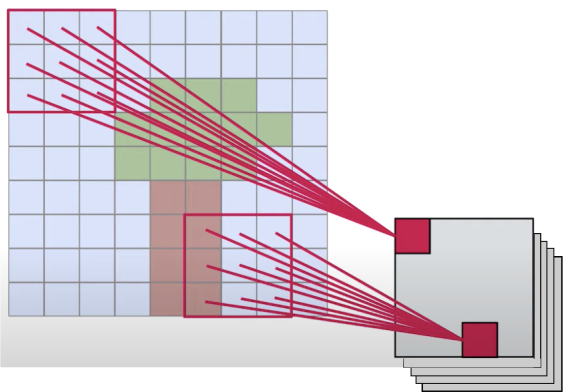
\includegraphics[height=0.4\textheight]{figures/convnet_v2.pdf}
  \end{center}
Convolutional layer.
\end{minipage}
\vfill
\scriptsize{Figures adapted from \citem{dieleman2020}.}\\
\vsp
\vsp
\normalsize{Check out more animated illustrations:}
\begin{itemize}
\item \link{https://github.com/vdumoulin/conv_arithmetic}\\
\item \link{https://cs231n.github.io/convolutional-networks/}
\end{itemize}
Also: lecture by Sander Dieleman (Deepmind) at UCL, London:
\link{https://www.youtube.com/watch?v=shVKhOmT0HE&feature=youtu.be}

\end{frame}

\begin{frame}{Convolutional layers, operation}
\vspace{-3mm}
Let $C$, $H$, $W$, $C'$, $H'$, $W'$, $d_{1}$, $d_{2}$ denote positive integers.\\
Description for 2D case. 2D convolutional layer:
\vsp
\begin{itemize}
\item \textbf{input}: image-like tensor $x$ with shape ($C$, $H$, $W$) (let's omit batch for now)
\item  \textbf{output}: also image-like $y$ with shape ($C'$, $H'$, $W'$), called \textit{feature map}
\item \textbf{model parameters}: weights and biases!
\begin{itemize}
\item ConvNets have $C'$ \emphbf{kernels}/\emphbf{filters} (vs.~Linear layers' weight matrix).
\item[-] $C'$ = number of output channels
\item Each kernel is a tensor of size ($C$, $d_{1}$, $d_{2}$). Here let's assume square kernels $d=d_1=d_2$. They are small ``image templates''.
\item bias $b \in \mathbb{R}^{C'}$ 
\end{itemize}
\end{itemize}
\vsp
\vsp
\pause
 Given \textbf{input} $x \in \mathbb{R}^{C \times H \times W}$, for each each output channel $ 1 \leq k \leq C'$, \textbf{output} $y_{k, i, j}$ ($ 1 \leq i \leq H'$, and $ 1 \leq j \leq W'$) is computed using the corresponding \textbf{kernel} $f^{(k)}$ of size $d$ (i.e.\, $f^{(k)} \in \mathbb{R}^{C \times d \times d}$):
\[
y_{k, i, j} =  \sigma\left(b_{k} + \sum_{c=1}^{C} \sum_{i'=i}^{i+d-1} \sum_{j'=j}^{j+d-1} f^{(k)}_{c, i'-i+1, j'-j+1} \times x_{c, i', j'}\right)
\]
\end{frame}

\begin{frame}{Convolutional layers, operation (cont'd)}
% Given \textbf{input} $x \in \mathbb{R}^{C \times H \times W}$, for each each output channel $ 1 \leq k \leq C'$, \textbf{output} $y_{k, i, j}$ ($ 1 \leq i \leq H'$, and $ 1 \leq j \leq W'$) is computed using the corresponding \textbf{kernel} $f^{(k)}$ of size $K$:
%\[
%y_{k, i, j} =  \sigma\left(b_{i,j} + \sum_{c=1}^{C} \sum_{i'=i}^{i+K-1} \sum_{j'=j}^{j+K-1} f^{(k)}_{c, i'-i+1, j'-j+1} \times x_{c, i', j'} \right)
%\]
\begin{itemize}
\item Indices make it look complicated, but it is not!\\
 We are sliding each kernel on the input image.\\
See e.g. \link{https://github.com/vdumoulin/conv_arithmetic/blob/master/gif/no_padding_no_strides.gif}
\item At each position, for each kernel, we are simply
computing the \textbf{dot product} (similarity measure) between the kernel and the input image within the local window.
\item Some terminologies: 
\begin{itemize}
\item[-] Locally connected (as opposed to fully connected)
\item[-] Weight sharing (across positions).
\end{itemize}
\item Note: computing a similarity between two ``vectors" using dot product is a fundamental concept (we will also see this for computing \textit{attention}). 
\end{itemize}
\end{frame}

\begin{frame}{Convolutional layers, specifications}
\vspace{-5mm}
To fully define the convolutional layer, we have to specify:
\begin{itemize}
\item number of input/output channels
\item kernel size
\item padding: how many "zeros" (or ones?) do we add on the borders to adjust the output ``image" size?\\
\link{https://github.com/vdumoulin/conv_arithmetic/blob/master/gif/same_padding_no_strides.gif}
\item stride: how many positions do we skip when we move the kernel over the image? also influence output size.\\
\link{https://github.com/vdumoulin/conv_arithmetic/blob/master/gif/padding_strides.gif}
\end{itemize}
See options in PyTorch \codeb{nn.Conv2d}. No need to overthink.
\begin{figure}
\centering
\includegraphics[width=.8\linewidth]{./figures/conv2d_pytorch.png}
\end{figure}
\end{frame}

\begin{frame}{More options in \codeb{nn.Conv2d} (excursion)}
\begin{itemize}
\item \code{groups}: number into which the input and output channels will be grouped.\\
Each group processed by different set of kernels.\\
\textit{grouped convolution (right)} with its equivalent with parallel convolution pipelines (left):
\begin{figure}
\centering
\includegraphics[width=.6\linewidth]{./figures/grouped_conv.png}
\end{figure}
Figure from \citem{XieGDTH17}. Idea used already in \citem{KrizhevskySH12}.
\vsp
\item \code{dilation}: spacing between kernel elements. For \textit{dilated convolution}.\\
See \link{https://github.com/vdumoulin/conv_arithmetic/blob/master/gif/dilation.gif}.
Got popular for audio processing \citem{oord2016wavenet}.
\end{itemize}
\end{frame}


%\begin{frame}{Convolutional neural networks,\\ recap jargon}
%\begin{itemize}
%\item Kernel\\
%(kernel is a quite overloaded term in ML...)
%\item Receptive field
%\item Feature map...
%\end{itemize}
%\end{frame}

\begin{frame}{Pooling layer}
 \vspace{-4mm}
\begin{itemize}
\item \textbf{input}: image $x$ with shape ($C$, $H$, $W$).
\item  \textbf{output}: also image $y$ with shape ($C'$, $H'$, $W'$). But smaller than $x$.
\item Operation: take max/mean over small, local sliding window to reduce image resolution (\emphbf{downsampling}).
\item \textbf{Allows to reduce computation for the following layer.}
\item \textbf{No model parameter}. Just a max/mean operation.
\item Hyper-parameter: as for convolution, need to specify pooling window dimensions, and how to move the window (stride).
\end{itemize}
\begin{figure}
                        \centering
                        \includegraphics[width=.65\linewidth]{./figures/max-pool-better.png}
% \vspace{-3mm}
\end{figure}
\scriptsize{Figure taken from \citem{stanford2019cnn}.}
%For example, pooling by factor 2:
%\[
%y_{k, i, j} = \max_{\substack{ 2 * i \leq i' \leq 2 * (i+K-1),\\  j \leq 2 * j' \leq 2 * (j+K-1)}}  x_{k, i', j'}
%\]
%where $K$ is the window size. Check indices!
%Note: Convolutional layer (with stride $\geq 2$) can also do downsampling. Convolution can be learned, but max-pooling is cheaper.
\end{frame}

\begin{frame}[fragile]{PyTorch examples}
\begin{itemize}
\item \codeb{nn.Conv2d} layer:
\begin{itemize}
\item Check input/output \textbf{shapes}!
\end{itemize}
\end{itemize}
\begin{python}
>>> input = torch.randn(16, 3, 48, 48)  # (B, C, H, W)
>>> layer = nn.Conv2d(3, 32, 3)  # default padding=0
>>> layer.weight.shape
torch.Size([32, 3, 3, 3])
>>> layer.bias.shape
torch.Size([32])
>>> output = layer(input)
>>> output.size()
torch.Size([16, 32, 46, 46])
>>> layer = nn.Conv2d(3, 32, 3, padding=1)
>>> output = layer(input)
>>> output.size()
torch.Size([16, 32, 48, 48])
>>> # it's flexible:
>>> layer = nn.Conv2d(3, 32, (3, 5), stride=(2, 1), padding=(1, 2))
>>> output = layer(input)
>>> output.size()
torch.Size([16, 32, 24, 48])
\end{python}
\end{frame}

\begin{frame}[fragile]{PyTorch examples (cont'd)}
\begin{itemize}
\item Max pooling layer: \codeb{nn.MaxPool2d}
\end{itemize}
\begin{python}
>>> input = torch.randn(16, 3, 48, 48)  # (B, C, H, W)
>>> pooling = nn.MaxPool2d(3)
>>> # non-overlapping pooling w/ window size (3, 3)
>>> output = pooling(input)
>>> output.size()  # 48 / 3 = 16
torch.Size([16, 3, 16, 16]) 
>>> # overlapping pooling w/ stride (2, 2)
>>> pooling = nn.MaxPool2d(3, stride=2)
>>> output = pooling(input)
>>> output.size()
torch.Size([16, 3, 23, 23])
>>> pooling = nn.MaxPool2d(3, stride=2, padding=1)
>>> # same as stride=(2, 2), padding=(1, 1)
>>> output = pooling(input)
>>> output.size()
torch.Size([16, 3, 24, 24])
>>> # downsampling by a factor 2 using a window size 3.
\end{python}
\end{frame}


\begin{frame}[fragile]{Put them together}
\vspace{-5mm}
ConvNets are obtained by alternating convolutional and pooling layers:
\begin{python}
class ConvNet(nn.Module):
    def __init__(self):  # just example.
        super(ConvNet, self).__init__()
        self.conv1 = nn.Conv2d(3, 6, 5)  # input shape (3, 32, 32).
        self.pool = nn.MaxPool2d(2, 2)
        self.conv2 = nn.Conv2d(6, 16, 5)
        self.fc1 = nn.Linear(16 * 5 * 5, 128)
        self.fc2 = nn.Linear(128, 64)
        self.fc3 = nn.Linear(64, 10)  # 10 output classes.

    def forward(self, x):
        x = self.pool(F.relu(self.conv1(x)))  # conv, pool.
        x = self.pool(F.relu(self.conv2(x)))  # conv, pool.
        x = x.view(-1, 16 * 5 * 5)  # linearlize input "images".
        x = F.relu(self.fc1(x))  # fully connected.
        x = F.relu(self.fc2(x))  # fully connected.
        x = self.fc3(x)  # fully connected.
        return x
\end{python}
\end{frame}

% \begin{frame}{Convolutional neural networks,\\  variants}
% There are many extensions/variants to convolutional neural networks...
% \begin{itemize}
% \item Dilated convolution \citem{YuK15}
% \item Depthwise-separable convolution \citem{Chollet17}
% \item ...
% \end{itemize}
% \end{frame}

\begin{frame}{So, shall we put more layers?}
\begin{itemize}
\item Observation (all figures from \citem{HeZRS16slides}):
\end{itemize}
\begin{figure}
\centering
\includegraphics[width=.65\linewidth]{./figures/no_resnet.png}
\end{figure}
\begin{itemize}
\item More layers should never hurt? If they learn identity in the worst case!
\end{itemize}
\begin{minipage}{0.45\textwidth}
\begin{center}
    \includegraphics[height=0.35\textheight]{figures/plain_net.png} \\
Standard network.
\end{center}
\end{minipage}
\begin{minipage}{0.45\textwidth}
\begin{center}
    \includegraphics[height=0.3\textheight]{figures/resnet.png}\\
Residual block.
\end{center}
\end{minipage}
\vsp
\begin{itemize}
\item Alternative intuition: simply inspired by LSTM-RNN (up next!).
\end{itemize}
\end{frame}

\begin{frame}{Very Deep NNs with skip connections}
\begin{itemize}
\item \emphbf{Skip connections}:
if a layer applies transformation $F$ to $x$ to get $y = F(x)$,
directly ``connect" $x$ to $y$ by skipping the transformation.
\item Two types:
\begin{itemize}
\item  \emphbf{Highway connection/networks} \citem{NIPS2015_5850} from \textbf{IDSIA}.\\
Gated connection like in LSTM (next subsection!):\\
$y = F(x) \odot g(x)+ x \odot h(x) $, \\
where $\odot$ denotes element-wise multiplication and the \textit{gates} $g$ and $h$ are neural networks.\\
\item \emphbf{Residual connection/networks} \citem{HeZRS16}. \\
Simple addition:
$y = F(x) + x $
\end{itemize}
\end{itemize}
\hspace{-10mm}
{\raggedleft
    \includegraphics[height=0.09\textheight]{figures/deep_net.png} \\
}
\begin{itemize}
\item Enable training models with more than 1000 layers in image recognition.
\item Also used in Transformer architectures (see later...)
\end{itemize}
\end{frame}

\begin{frame}{Skip connections, performance}
\begin{itemize}
\item 
ImageNet Large Scale Visual Recognition Competition (ILSVRC) top-5 error (\%) (from \citem{HeZRS16slides}):
\end{itemize}
\begin{figure}
\centering
\includegraphics[width=.5\linewidth]{./figures/image_net.png}
\end{figure}
\begin{itemize}
\item Many follow up works... 
\begin{itemize}
\item By the same authors: improved resblocks \citem{HeZRS16b} (deeper)
\item Wide residual nets \citem{ZagoruykoK16}
\item DenseNets \citem{HuangLMW17, lang1988learning}...
\end{itemize}
\end{itemize}
\end{frame}

\begin{frame}{Convolutional neural networks,\\
beyond images}
\textbf{Applications beyond image processing}:
\begin{itemize}
\item Natural language: e.g.
\begin{itemize}
\item Text classification \citem{kim2014convolutional}
\item Machine translation \citem{GehringAGYD17}
\end{itemize}
\item Speech recognition \citem{waibel1989phoneme}
\end{itemize}\vsp
... and much more. We could have done the whole lecture on ConvNets...\\
\vsp
\textbf{From engineering view point,}
\begin{itemize}
\item Like pooling layers, convolutional layers (with stride $\geq 2$) allow us to downsample the input (reduce input resolution).
\item  It's a general tool for trainable downsampling (e.g.
reduce a long sequence to a shorter one).
\item Convolution can be learned vs. max-pooling is parameter-free and cheap.
\end{itemize}
Interested in historical background? Watch Prof. Schmidhuber's video: \link{https://youtu.be/ysOw6lNWx2o?t=20}
\end{frame}

\begin{frame}{Exercise 5 / Assignment 2}
	A few words on \emphbf{Assignment 2}:
	\begin{itemize}
		\item You will be building a full pipeline for image classification using
        \item[-] convolutional neural networks
        \item[-] some practical training tricks
		\item Remember the usual workflow (Chapter 1)!
        \item Similar task in Exercise 4
	\end{itemize}
\end{frame}